%\documentclass[tikz, border=5pt]{standalone}
\begin{document}
	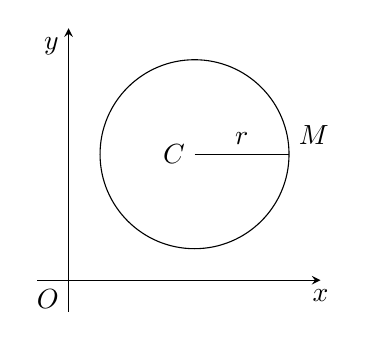
\begin{tikzpicture} [>=stealth, scale=0.8]
		% 1. 绘制坐标轴
		\draw[->] (-0.5,0) -- (4,0) node[below] {$x$};  % x轴
		\draw[->] (0,-0.5) -- (0,4) node[below left] {$y$};  % y轴
		\node at (0,0) [below left] {$O$};  % 标记原点
		
		% 2. 绘制圆(圆心C(2,2),半径1.5)
		\draw (2,2) circle (1.5);
		\node at (2,2) [ left] {$C$};  % 标记圆心
		
		% 3. 绘制半径线段CM并标记
		\draw (2,2) -- (3.5,2) node[midway, above] {$r$};  % 半径线段
		\node at (3.5,2) [above right] {$M$};  % 标记圆上点M
		
	\end{tikzpicture}
\end{document}
